\begin{Ueberlieferung}% 
{\textit{L}}Aufzeichnung: LH XXXVIII Bl. 24.
1 Bl. 4\textsuperscript{o}.
1 S. auf Bl. 24~r\textsuperscript{o}. Bl. 24~v\textsuperscript{o} leer.
Papier\-ränder besch\"{a}digt, ohne Textverlust.
Haupttext und Marginalien sind durch die Zeich\-nung [\textit{Fig.~1}] voneinander getrennt.
\newline%
Cc 2, Nr. 1133 B
\end{Ueberlieferung}
%
%\begin{Datierungsgruende}%
%Siehe Einleitung zu N. ???.
%\end{Datierungsgruende}
%
%  
\count\Afootins=1200
\count\Bfootins=1200
\count\Cfootins=1200  
\newpage                
\pstart
\noindent%
% [24~r\textsuperscript{o}]
\noindent%
[24~r\textsuperscript{o}]
\edtext{Il y a 3 pouces de saut\protect\index{Sachverzeichnis}{saut} \`{a} tous ces endroits, $A$, $B$, $C$,
distance \`{a} peu pres d'un quart de lieue, ou de 7 ou 800 toises;
elle a 4 pieds de haut aux moindres endroits; s\c{c}auuoir deux choses:}%
{\lemma{\textit{Neben der Zeichnung:}}\Afootnote{%
Bouchons\textsuperscript{[a]}
14 toises de large sur deux d'ouuerture ou $\displaystyle\frac{1}{8}^{me}$\textsuperscript{[b]}
on trouue cela commode dans l'experience pour juger de la\textsuperscript{[c]}
vitesse, il faut\textsuperscript{[d]}\\ 
\vspace*{2mm}\footnotesize%
\textsuperscript{[a]} Bouchons \textit{erg. L}%
\quad%
\textsuperscript{[b]} ou $\displaystyle\frac{1}{8}^{me}$ \textit{erg. L}%
\quad%
\textsuperscript{[c]} la \textbar\ pente\protect\index{Sachverzeichnis}{pente} par la \textit{gestr.} \textbar\ vitesse, \textit{L}%
\quad%
\textsuperscript{[d]} faut [\textit{Text bricht ab.}]}} 
\newline\indent
1. en ostant une digue\protect\index{Sachverzeichnis}{digue} ou barre\protect\index{Sachverzeichnis}{barre} comme
\edtext{cela,%
\edtext{}{\lemma{\textit{Neben der Zeichnung:}}\Afootnote{%
Cela sert pour diminuer l'inondation\protect\index{Sachverzeichnis}{inondation} des rivieres,\protect\index{Sachverzeichnis}{riviere}
en ostant des barres\protect\index{Sachverzeichnis}{barre}.\vspace*{2mm}}}
%
[où] (+~pertuis\protect\index{Sachverzeichnis}{pertuis} c'est le trou~+) l'eau baissera}%
{\lemma{cela,}\Bfootnote{\textbar\ ou \textit{ändert Hrsg.} \textbar\ %
\textit{(1)}\ pertuis; %
\textit{(2)}\ (+~pertuis c'est le trou~+) %
\textit{(a)}\ s\c{c}auoir
\textit{(b)}\ l'eau baissera \textit{L}}}
(\phantom)\hspace{-1.2mm}+~dans un 4\textsuperscript{t} de lieue:
nous adjoutant trois pouces de
\edtext{pente dans ce quart de lieue~\phantom(\hspace{-1.2mm}+)
s\c{c}auuoir}{\lemma{pente}\Bfootnote{%
\textit{(1)}\ dans tout ce corps %
\textit{(2)}\ dans [...] lieue~\phantom(\hspace{-1.2mm}+) %
\textit{(a)}\ Il vient une crue d'eau qui %
\textit{(b)}\ s\c{c}auuoir \textit{L}}}
\edtext{combien elle baissera au pied de la superieure.
C'est \`{a} dire en ostant la digue\protect\index{Sachverzeichnis}{digue} $N,$
combien l'eau baissera au dessous de la}%
{\lemma{\textit{Neben der Zeichnung:}}\Afootnote{%
Le vent d'un double de vistesse, fera un effect quadruple, et l'eau de m\^{e}me.\textsuperscript{[a]}
La m\^{e}me eau qui tombe de deux pieds de haut, cela augmente la vistesse seulement, et non pas la matiere.
Ergo vires erunt ut cubi potius.\\%
\vspace*{2mm}\footnotesize%
\textsuperscript{[a]} m\^{e}me. \textit{(1)}\ L'eau qui tombe \textit{(2)}\ La m\^{e}me eau qui tombe \textit{L}}}
%
\edtext{digue\protect\index{Sachverzeichnis}{digue} $M$.
Quand}{\lemma{digue $M$.}\Bfootnote{%
\textit{(1)}\ Combien la 2\textsuperscript{de}, la 3\textsuperscript{me} %
\textit{(2)}\ 2. deux b
\textit{(3)}\ Quand \textit{L}}}
on oste les barres\protect\index{Sachverzeichnis}{barre} $M.$ $N.$
l'eau baissera davantage \`{a} $L$, qu'elle n'avoit fait \`{a} $M$, ostant $N$ seulement,
et on demande la proportion, jusqu'en ostant toute celle d'en haut.
\newline\indent 
\edtext{2. d'une crue d'eau, qui augmente la riviere\protect\index{Sachverzeichnis}{riviere} de 4 pieds de haut
(+~les sauts\protect\index{Sachverzeichnis}{saut} alors deviennent beaucoup plus grands,~+)}%
{\lemma{\textit{Neben der Zeichnung:}}\Afootnote{%
Experiences\protect\index{Sachverzeichnis}{experience} \`{a} faire:
une eau de telle pente, et de telle epais\-seur, à une telle vitesse, il faut pour cela un canal.\vspace{-4mm}}}
%
on demande toutes les barres\protect\index{Sachverzeichnis}{barre} estant ost\'{e}es
combien l'enflure en seroit elle
\edtext{moindre. Il y a peu de pente et par consequent l'eau}%
{\lemma{moindre.}\Bfootnote{\textit{(1)}\ L'eau %
\textit{(2)}\ Il y [...] l'eau \textit{L}}}
va lentement dans une telle riviere\protect\index{Sachverzeichnis}{riviere},
o\`{u} il y a le m\^{e}me saut.\protect\index{Sachverzeichnis}{saut}
Quand il vient une crue d'eau de 4 
\edtext{pieds la pente}%
{\lemma{pieds}\Bfootnote{\textit{(1)}\ d'eau %
\textit{(2)}\ la pente \textit{L}}}
devient plus grande de 4 pieds, et l'epaisseur aussi et par consequent la vistesse par 2 raisons.
\pend 
\newpage
\pstart 
\centering
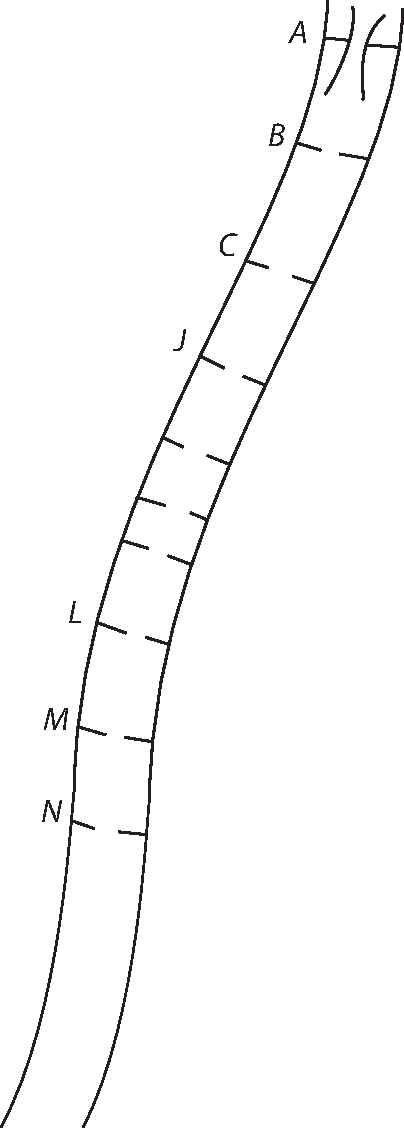
\includegraphics[width=0.33\textwidth]{images/LH038_24r-d.pdf}
\pend
\vspace{3mm}
\pstart
\centering [\textit{Fig. 1}]
\pend
\newpage
\count\Afootins=1500
\count\Bfootins=1500
\count\Cfootins=1500
 


 


 


 


 


 

